\label{sec:hessian}

%\rnote{Title of this section is a bit long and don't have a real focus. We might consider break it into multiple sections? One possibility is that we talk about the decomposition, then talk about properties of $xx^T$ (both zero-mean and non-zero-mean case) and briefly talk about properties of $M$ (mostly empirical); in the next section we can then use this decomposition to justify (a) Hessian overlap; (b) low rank structure of the top eigenvectors; (c) rank C-1 Hessian}

The fact that layer-wise Hessian for fully connected layers can be decomposed into the expectation of Kronecker products as in \cref{eqn:decomp} poses a natural question: Can the Hessian be approximated using the Kronecker product of the expectations? That is, whether 
\begin{equation}
    \HessL^{(p)}(\theta) = \E\left[\mM\otimes \vx\vx^T\right] \approx \E[\mM] \otimes \E[\vx\vx^T]. 
\end{equation}

We call the above conjecture ``the decoupling conjecture''. Equivalently, we conjecture that the two matrices $\mM$ and $\vx\vx^T$ are approximately statistically independent.

%\rnote{Maybe we should call the above a conjecture with a name (something like ``the decoupling conjecture''?), then we say that empirically we show the conjecture is true, and this has a lot of benefits.}

If this conjecture is true, we can analyze the layer-wise Hessian by analyzing the two components separately. Note that $\E[\mM]$ is the Hessian of the layer-wise output with respect to empirical loss, and $\E[\vx\vx^T]$ is the auto-correlation matrix of the layer-wise inputs. For simplicity we call $\E[\mM]$ the output Hessian and $\E[\vx\vx^T]$ the input auto-correlation.

As both $\E[\mM]$ and $\E[\vx\vx^T]$ can be computed in time comparable to back-propagation, algorithm then provides us with a fast inference of second order information. Also, explicit calculation of the layerwise Hessian requires $O(m^2n^2)$ space but our approximation only requires $O(m^2+n^2)$ space.

Moreover, we can approximate the eigenvectors and eigenvalues of the layer-wise Hessian $\HessL^{(p)}(\theta)$ by $\E[\mM]$ and $\E[\vx\vx^T]$. Let $\vm$ and $\vv$ be an eigenvector of $\E[\mM]$ and $\E[\vx\vx^T]$ respectively, with corresponding eigenvalues $\lambda_\vm$ and $\lambda_\vv$. Since both matrices are positive semi-definite, $\vm \otimes \vv$ is an eigenvector of $\E[\mM] \otimes \E[\vx\vx^T]$ with eigenvalue $\lambda_\vm\lambda_\vv$. In this way, since $\E[\mM]$ has $n$ eigenvectors and $\E[\vx\vx^T]$ has $m$ eigenvectors, we can approximate all $mn$ eigenvectors for the layerwise Hessian.

Similar approximation for Fisher Information matrices have been used in K-FAC \citep{martens2015optimizing}. While they give efficient calculation for the matrix inverse, our analysis focuses more on the structural analysis. Besides, unlike K-FAC, we can calculate top eigenvalues and eigenvectors of the Hessian efficiently \citep{yao2019pyhessian} so that the approximation of top eigenspace can be directly compared. \ynote{Put in for comparison, can be deleted}

For convolutional layers (convs), we propose a similar Kronecker factorization motivated by \citet{grosse2016kronecker}. We also denote it as $\E[\mM]\otimes \E[\vx\vx^T]$ but with a different definition of $\mM$.(See \cref{sec:appendix_conv} for details) \ynote{Where should we put this paragraph?}\cnote{I think it's ok to put it here.}
\subsection{Hessian Approximation}
We conduct experiment on CIFAR-10 \citep{Krizhevsky09learningmultiple} and MNIST \citep{lecun1998gradient} dataset using several different Fully Connected (FC) networks, several variations of LeNet \citep{lecun1998gradient}, and VGG11 \citep{simonyan2014very}. The results shown in the main text are variants of LeNet5 trained on CIFAR-10 and FC2 trained on MNIST. Other representative results are shown in \cref{sec:appendix_exp_res}. The eigenvalues and eigenvectors of the exact layer-wise Hessians are approximated using a modified Lanczos algorithm, which is described in detail in \cref{sec:appendix_eigencomp}.

To verify the validity of the approximation, we compare the eigenvalues and top eigenspaces of the approximated Hessian and the true Hessian.
We define the dimension $k$ top eigenspace of a matrix as the subspace spanned by the eigenvectors corresponding to its $k$ largest eigenvalues.

\theoremstyle{definition}
\begin{definition}[Subspace Overlap]
For $k$-dimensional subspaces $\mU,\mV$ in $\R^d$ ($d\geq k$) where the basis vectors $\vu_i$s and $\vv_i$s are column vectors, with $\vtheta$ as the size $k$ vector of canonical angles between $\mU$ and $\mV$, we define the subspace overlap of $\mU$ and $\mV$ as
\begin{equation}
    \Overlap(\mU, \mV) := \frac{1}{k}\|\mU^T\mV\|^2_F =\frac{1}{k}\|\cos\vtheta\|^2.
    \label{eqn:overlap}
\end{equation}
\end{definition}

For two $k$-dimensional subspaces in the same space,
we define the subspace overlap as the L2 average of the cosine of canonical angles: For $k$-dimensional subspaces $\mU,\mV$ in $\R^d$ ($d\geq k$) where the basis vectors $\vu_i$s and $\vv_i$s are column vectors. . we define the subspace overlap of $\mU$ and $\mV$ as
\begin{equation}
    \Overlap(\mU, \mV) := \frac{1}{k}\|\mU^T\mV\|^2_F =\frac{1}{k}\|\cos\vtheta\|^2,
    \label{eqn:overlap}
\end{equation}
Note that when $k=1$, the overlap is equivalent to the dot between the two vectors. This definition is equivalent to the definition in \citet{gur2018gradient}.(Proof shown in appendix\cnote{Remember to specify which part of appendix})

Empirical results show that this approximation works reasonably well, especially for the top eigenvalues and eigenspace, as shown in \cref{fig:approx_result}. The eigenvectors are ranked in the order of decreasing eigenvalues, and the overlap at dimension $k$ is the overlap of subspaces consist of top $k$ eigenvectors. 

\begin{figure}[th]
    \centering
    \begin{subfigure}[b]{0.5\textwidth}
        \centering
        \captionsetup{justification=centering}
        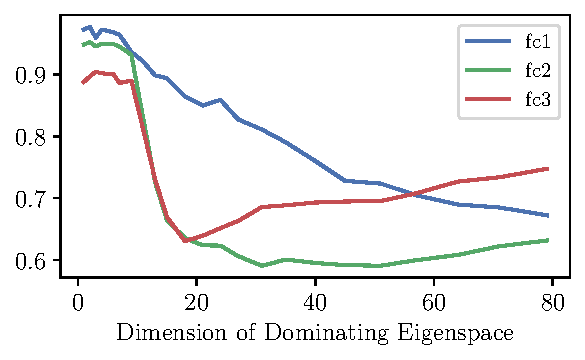
\includegraphics[width=\textwidth]{Figures/ApproxQuality/FC2_fixlr/sample_kron_decomp_traceoverlap_d80_MNIST_Exp1_FC2_fixlr0.01R2_E-1.pdf}
        \caption{Subspace overlap between\\ approximated and exact layer-wise hessian}
        \label{fig:overlap_approx}
    \end{subfigure}%
    \begin{subfigure}[b]{0.5\textwidth}
        \centering
        \captionsetup{justification=centering}
        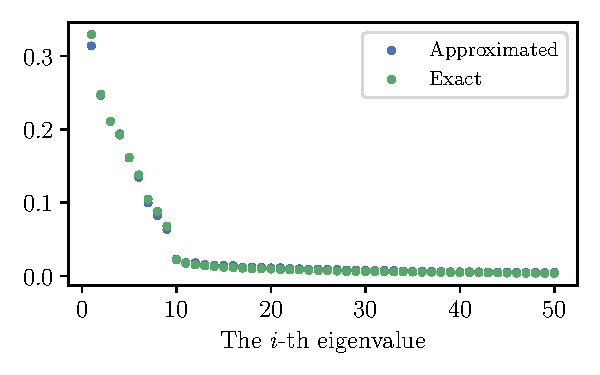
\includegraphics[width=\textwidth]{Figures/ApproxQuality/FC2_fixlr/eigenval_compare_top50_MNIST_Exp1_FC2_fixlr0.01R2_E-1_fc2.pdf}
        \caption{Top eigenvalues of approximated\\ and exact layer-wise Hessian for fc2-FC2}
        \label{fig:eigenval_approx}
    \end{subfigure}
    \caption{FC2 MNIST \znote{To be completed}}
    \label{fig:approx_result}
\end{figure}
\subsection{Eigenvector Correspondence}
\label{sec:eigen_corr}
\begin{figure}[ht]
    \centering
    \begin{subfigure}[t]{0.46\textwidth}
        \centering
        \captionsetup{justification=centering}
        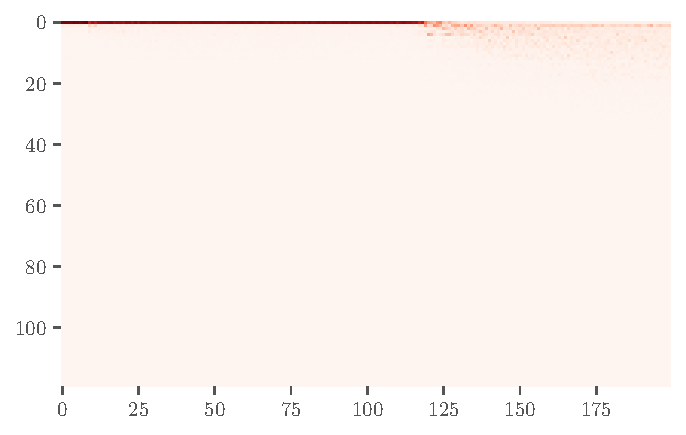
\includegraphics[width=\textwidth]{Figures/Correspondence/LeNet5_fixlr0.01/xxT_Trueest_real_corr_expand_t200_CIFAR10_Exp1_LeNet5_fixlr0.01R2_E-1_fc1.pdf}
        \caption{True Hessian with $\E[\vx\vx^T]$}
        \label{fig:Corr_xxT_True_fc}
    \end{subfigure}%
    \begin{subfigure}[t]{0.46\textwidth}
        \centering
        \captionsetup{justification=centering}
        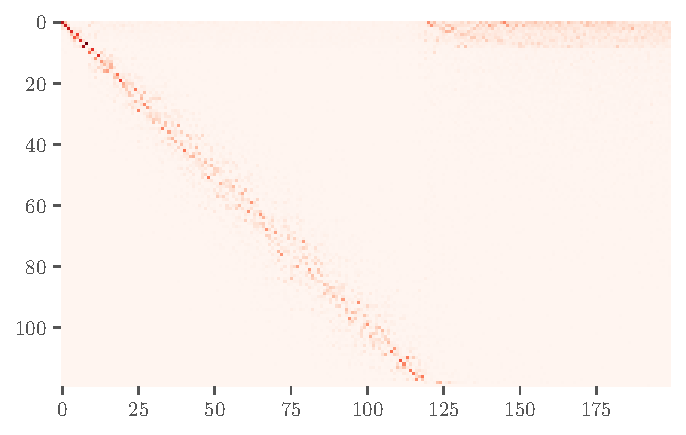
\includegraphics[width=\textwidth]{Figures/Correspondence/LeNet5_fixlr0.01/UTAU_Trueest_real_corr_expand_t200_CIFAR10_Exp1_LeNet5_fixlr0.01R2_E-1_fc1.pdf}
        \caption{True Hessian with $\E[\mM]$}
        \label{fig:Corr_UTAU_True_fc}
    \end{subfigure}%
    \begin{subfigure}[t]{0.065\textwidth}
        \centering
        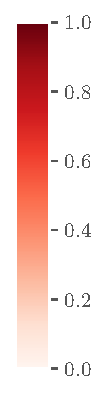
\includegraphics[width=\textwidth]{Figures/Misc/colorbar.pdf}
    \end{subfigure}
    \bigskip
\begin{subfigure}[t]{0.46\textwidth}
        \centering
        \captionsetup{justification=centering}
        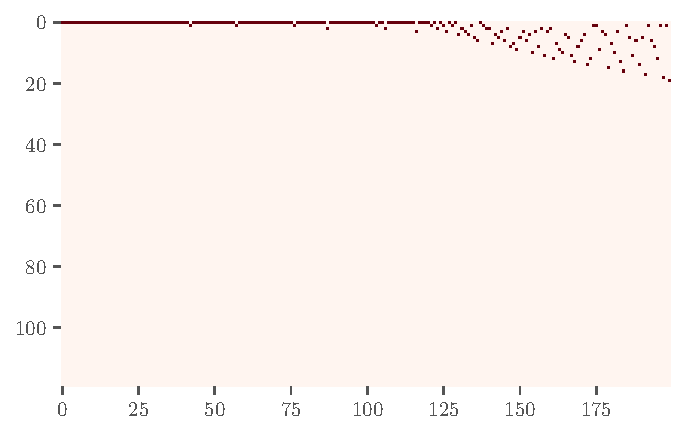
\includegraphics[width=\textwidth]{Figures/Correspondence/LeNet5_fixlr0.01/xxT_Approxest_real_corr_expand_t200_CIFAR10_Exp1_LeNet5_fixlr0.01R2_E-1_fc1.pdf}
        \caption{Approximated Hessian with $\E[\vx\vx^T]$}
        \label{fig:Corr_xxT_Approx_fc}
    \end{subfigure}%
    \begin{subfigure}[t]{0.46\textwidth}
        \centering
        \captionsetup{justification=centering}
        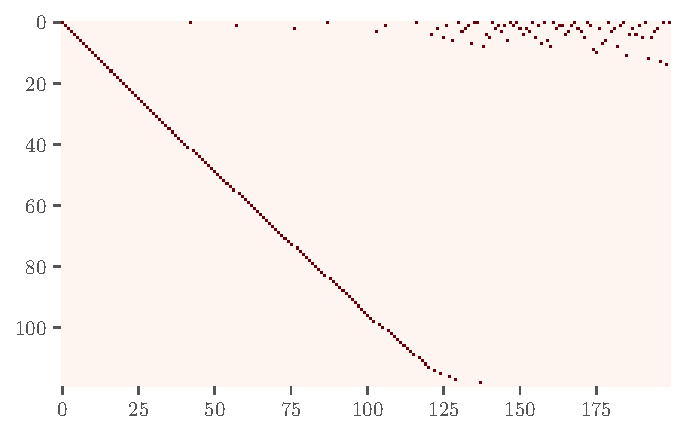
\includegraphics[width=\textwidth]{Figures/Correspondence/LeNet5_fixlr0.01/UTAU_Approxest_real_corr_expand_t200_CIFAR10_Exp1_LeNet5_fixlr0.01R2_E-1_fc1.pdf}
        \caption{Approximated Hessian with $\E[\vx\vx^T]$}
        \label{fig:Corr_UTAU_Approx_fc}
    \end{subfigure}%
    \begin{subfigure}[t]{0.065\textwidth}
        \centering
        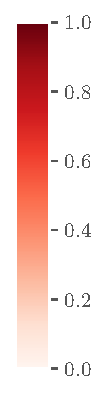
\includegraphics[width=\textwidth]{Figures/Misc/colorbar.pdf}
    \end{subfigure}
    \caption{Eigenvector Correspondence for fc1 in LeNet5 ($n$=120)}
    \label{fig:Corr_fc_approx}
\end{figure}
To better visualize how eigenvectors of layer-wise Hessian are correlated with eigenvectors of $\E[\mM]$ and $\E[\vx\vx^T]$, we introduce `eigenvector correspondence matrices' as shown in \cref{fig:Corr_fc_approx}. Take $\E[\vx\vx^T]$ as an example. Let $\vv_i$ be the $i$th eigenvector of $\E[\vx\vx^T]$ and $\vh_j$ be the $j$th eigenvector of layer-wise Hessian, both ranking in decreasing order of eigenvalues. We can then define $\Krsp(\vv_i)$ as the $n$ dimensional subspace of $\vv_i$'s Kronecker products in $\R^{mn}$ where $\vh_j$ lives in.\cnote{It's still confusing to me if you say ``one's Kronecker products'' because Kronecker product is a binary operator, perhaps use ``one's Kronecker products with xxx'' instead?} Columns of $\mI_n \otimes \vv_i$ form the basis for $\Krsp(\vv_i)$. 
Since $\vh_j$ lives in the same space as the weight vector $\vw$ of that layer, we can define an operation $\Mat(\vh_i)$ to reshape $\vh_i$ into a matrix with the same shape as the weight matrix $\mW$. \ynote{Should we move this defintion of $\Mat$ to Section 3? Also we can choose one version of explanation between the subspace of Kronecker products and the reshape into the shape of weight matrix, but this may require a rephrase of all the explanations below in Seciton 4.}
\znote{Do we include this in a definition environment}

We can then define the correspondence between $\vv_i$ and $\vh_j$ as
\begin{equation}
    \Corr(\vv_i, \vh_j) = \|(\mI_n \otimes \vv_i)^T\vh_j\|^2 = \|\Mat(\vh_j)\vv_i\|^2,
\end{equation}
where 
Its value is shown in the $(i,j)$-entry of the heatmap. The eigenvector correspondence for $\E[\mM]$ is defined in the same way, except that the subspace for $\E[\mM]$'s $i$th eigenvector $\vm_i$ is $\vm_i \otimes \mI_m$. (Or $\|\Mat(\vh_j)^T\vm_i\|^2$ if we use the second definition.)

If $\Corr(\vv_i, \vh_j) \approx 1$, we have $\vh_j \approx \vu \otimes \vv_i$, with some $\vu \in \R^n$. \ynote{Or state $\Mat(\vh_j)^T = \vu\vv_i^T$, we can then omit this in \cref{sec:domin_eig} }We can also say $\vh_j \in \Krsp(\vv_i)$. From \cref{fig:Corr_fc} and \cref{fig:Corr_conv}, we can see that around $n$ top eigenvectors are in $\Krsp(\vv_1)$, where $\vv_1$ is the first eigenvector of $\E[\vx\vx^T]$. This leads us to analyze the structure of $\E[\vx\vx^T]$.
\cnote{I think this subsection is very hard for the readers to understand. My suggestion is to interpret our result in a reverse way, i.e., we first hypothesize that our approximation is totally accurate, then the top eigenvectors of Hessian should be the top eigenvector of $E[xx^T]$ Kronecker with the top eigenvectors of $E[M]$, and we design this method to test our hypothesis, and then show the figures. Besides, for the figures, I think we need more interpretations instead of letting the readers look at them directly. We can perhaps say ``We can see a diagonal pattern in Figure x, indicating that the $i$-th eigenvector of the layerwise Hessian indeed mainly comes from xxx''.} \ynote{There may be some differences because our explanation does not depend on the approximation is good for the E[M] part and we would like to present a more general model}

\subsection{Structure of Auto-correlation Matrix \texorpdfstring{$\E[\vx\vx^T]$}{ExxT}}
\label{sec:xxT}
From \cref{fig:xxT}, we can see $\E[\vx\vx^T]$ are all close to rank 1. This phenomenon is also observed along the training trajectory and in other networks.
\begin{figure}[th]
    \centering
    \begin{subfigure}[b]{0.33\textwidth}
        \centering
        \captionsetup{justification=centering}
        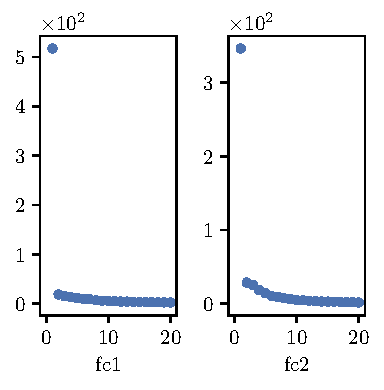
\includegraphics[width=\textwidth]{Figures/Eigenspectrum/xxT/xxT_sigval_d20_MNIST_Exp1_FC2_fixlr0.01R1_E-1_fc1fc2.pdf}
        \caption{Fully connected layers of FC2 (MNIST)}
        \label{fig:xxT_sig_fc2}%
    \end{subfigure}
    \hfill
    \begin{subfigure}[b]{0.33\textwidth}
        \centering
        \captionsetup{justification=centering}
        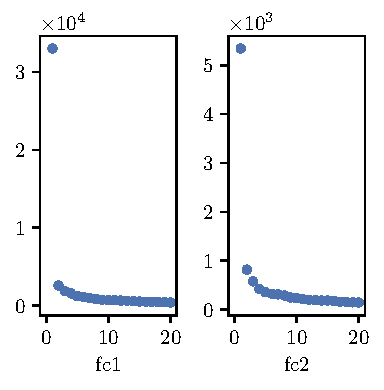
\includegraphics[width=\textwidth]{Figures/Eigenspectrum/xxT/xxT_sigval_d20_CIFAR10_Exp1_LeNet5_fixlr0.01R1_E-1_fc1fc2.pdf}
        \caption{Fully connected layers of LeNet5 (CIFAR10)}
        \label{fig:xxT_sig_lenet}
    \end{subfigure}%
    \hfill
    \begin{subfigure}[b]{0.33\textwidth}
        \centering
        \captionsetup{justification=centering}
        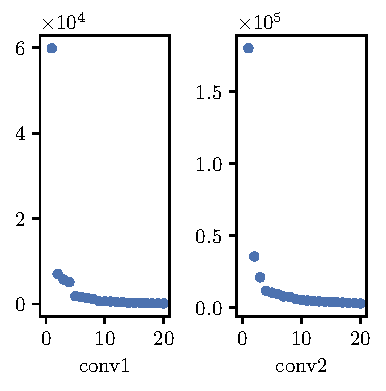
\includegraphics[width=\textwidth]{Figures/Eigenspectrum/xxT/xxTConv_sigval_d20_CIFAR10_Exp1_LeNet5_fixlr0.01_E-1.pdf}
        \caption{Convolution layers of LeNet5 (CIFAR10)}
        \label{fig:xxT_sig_lenet}
    \end{subfigure}
    \captionsetup{justification=centering}
    \caption{Eigenspectrum of $\E[\vx\vx^T]$ for different layers in different models. All are close to rank 1.\znote{This figure should go to appendix as there is not much useful information which specifically requires a graph to visualize}}
    \label{fig:xxT}
\end{figure}

Let the $\hE[\vx]$ be normalized $\E[\vx]$ for FCs and the first left singular vector of $\E[\vx]$ for conv. We also find that the top eigenvector of $\E[\vx\vx^T]$ ($\vv_1$) is almost equal to $\hE[\vx]$, as their inner product are usually larger than 0.998. This suggests that $\E[\vx]\E[\vx]^T$ approximately equals to $\E[\vx\vx^T]$ and dominates the covariance $\mSigma_\vx$. It is verified as the Spectral norm of $\E[\vx]\E[\vx]^T$ is more than 5 times that of $\mSigma_\vx$ in all our experiments. This is natural because $\vx$ are output of ReLU layers and thus nonnegative, for all layers other than the input layer.
 \rnote{We should just show the empirical observation that the covariance matrix has small spectral norm, therefore by standard matrix perturbation bounds the true matrix is still close to rank 1 and the top eigenvector is close to $\E[x]$}

\subsection{Further Approximation for the Top Eigenspace of Layerwise Hessian}
\label{sec:approx_top_eig}
Since the top eigenvector of $\E[\vx\vx^T]$, $\vv_1$ is approximately $\hE[\vx]$, with results in \cref{sec:eigen_corr}, around $n$ top eigenvectors of layer-wise Hessian are all in $\Krsp(\hE[\vx])$. 

Let the number of top eigenvectors of layerwise Hessian are approximated in $\Krsp(\hE[\vx])$ be $s$. In most cases as in \cref{fig:Corr_fc} and \cref{fig:Corr_conv}, $s \approx n$. Thus, for $i \leq s$, $i$th eigenvector $\vh_i \approx \vu_i \otimes \hE[\vx]$ for some $\vu_i \in \R^n$. Thus, for any $k \leq s$, the top $k$ eigenspace of the Hessian can be approximated as $\mU_k \otimes \hE[\vx]$, where columns of $\mU_k$ are $\vu_1, \ldots, \vu_k$.

Note that this approximation and most explanations in \cref{sec:empirical} does not depend on $\vv_1 \approx \hE[\vx]$ and as we can substitute $\vv_1$ for $\hE[\vx]$. We use $\hE[\vx]$ to show the identity of $\vv_1$ in most cases and give more intuition for the discussion.

\cnote{I fell like we are using too many formulas and a bit complicated notations, which will confuse the readers. Here perhaps we need to remind people what is Krsp and what is n. I think it's better to interpret things by words instead of formulas in the main text since this is not really a theoretical paper. For example, for the last sentence in the above paragraph, we can instead say ``Thus, the top $s$ eigenvectors of the Hessian can be well approximated by the Kronecker products between $E[x]$ and the top eigenvectors of $E[M]$.'' I would assume that people can only remember what is $M$ and $xx^T$, so perhaps we need to avoid using notations like $u_i$ if possible. Also, I think the use of ``temporary variables'' is not necessary in most of the texts. We can use English instead, and it also saves some space I guess. I mean, instead of saying ``$\forall i\leq s$'', we can say ``for the first $s$ eigenvectors of ...''}

Also, for some FC layers, the eigenvector correspondance heatmap of $\E[\mM]$ has a diagonal pattern in the first $s$ columns, as shown in \cref{fig:Corr_fc}. We can further approximate the $\vu_i$'s as the $i$th eigenvector of $\E[\mM]$. In this case, $\mU_k$ is the top $k$ eigenspace of $\E[\mM]$. There are also some cases where $s$ is considerably smaller than $n$, and larger than $n$ in rare cases. We will discuss them in the Appendix.